\documentclass[12pt,letterpaper]{article}

% ---------- Paquetes ----------
\usepackage[utf8]{inputenc}
\usepackage[T1]{fontenc}
\usepackage[spanish]{babel}
\usepackage{newtxtext}         % Fuente Times New Roman para el texto
\usepackage{newtxmath}
\linespread{1.05}
\usepackage[margin=2.5cm]{geometry}
\usepackage{enumitem}
\usepackage{graphicx}
\usepackage{caption}
\usepackage{microtype}
\usepackage{float}
\usepackage{xcolor}
\usepackage[normalem]{ulem}
\usepackage{xurl}
\usepackage{titlesec}
% ---------- Colores ----------
\definecolor{azullink}{RGB}{25,75,135}   %
\definecolor{azultitulo}{RGB}{0,0,0} 
\definecolor{azulmarino}{RGB}{10,35,80}
\newcommand{\azul}[1]{#1}                
% ---------- Links (azules y subrayados) ----------
\usepackage[colorlinks=true, urlcolor=azullink, linkcolor=black, citecolor=black]{hyperref}
\urlstyle{same}
\Urlmuskip=0mu plus 2mu
% ---------- Formato ----------
\setlength{\parindent}{0pt}
\setlength{\parskip}{6pt}
\setlist{itemsep=4pt}
\sloppy
\setlength{\emergencystretch}{3em}

% Formato automático para que los \section* salgan en azul marino y subrayados
\titleformat{\section}
  {\Large\bfseries\color{azulmarino}} 
  {}                                 % Sin numeración
  {0pt}                              % Separación
  {\uline}                           % Aplicar subrayado al texto
\begin{document}
% ---------- Título principal ----------
\begin{center}
\vspace*{0.5cm}
{\color{azultitulo}\rule{\textwidth}{1.5pt}}\par
\vspace{0.45cm}
{\Huge\bfseries\color{azultitulo} DEFINICIÓN Y ANÁLISIS\par}
\vspace{0.15cm}
{\LARGE\bfseries\color{azultitulo} DE UN PROBLEMA SISTÉMICO\par}
\vspace{0.3cm}
% Subtítulo en \Large, negrita, color azullink y subrayado con \uline
{\Large\bfseries\color{azullink}\uline{Análisis de la problemática laboral y estructural del IMSS en México}\par}
\vspace{0.45cm}
{\color{azultitulo}\rule{\textwidth}{1.5pt}}\par
\end{center}

\section*{Paso 1: La Semilla de la Indignación}

\textbf{Problema:} Desigualdad de clases sociales en México.

\textbf{Justificación sistémica:} Las manifestaciones recientes de los trabajadores del IMSS no solo se tratan de marchas o protestas, sino que reflejan problemas más profundos, como el desabasto de medicamentos, la falta de material médico, las condiciones laborales y la injusticia salarial. Es preocupante que quienes en algún momento fueron reconocidos como héroes durante la pandemia ahora tengan que enfrentar situaciones de explotación y trabajar con recursos insuficientes. Era cuestión de tiempo para que este descontento se hiciera evidente. No es posible brindar una atención médica adecuada si los hospitales no cuentan con los materiales y medicamentos esenciales para atender a los pacientes. Los trabajadores de la salud desempeñan un papel fundamental en nuestra sociedad, pues su labor puede marcar la diferencia entre la enfermedad y la recuperación, e incluso entre la vida y la muerte. Además, refleja un problema de desigualdad social, ya que mientras algunas personas pueden acudir a hospitales privados y pagar por una atención médica de calidad, muchas otras dependen de los servicios públicos de salud y se ven afectadas por la falta de medicamentos, materiales y recursos. Esto demuestra que el acceso a la salud no debería depender de la situación económica de cada persona, sino que tendría que ser un derecho garantizado para todos.

% =====================================================
\section*{Paso 2: Autopsia del Problema (Modelo del Iceberg)}

\subsection*{a) El Evento (La punta del iceberg): Mega marcha nacional del IMSS.}

El día 15 de octubre de 2026 los trabajadores del Instituto Mexicano del Seguro Social (IMSS) realizaron una marcha para exigir que el gobierno cumpla sus peticiones, entre ellas: un aumento de salario, ya que, en una consulta de salarios fueron rechazados al aumento del 2.9 por ciento al salario tabular, también exigen mejores instalaciones y más medicamentos, puesto que, ya no es suficiente para la cantidad de población que asiste a la institución pública.

Merino, F. (2026, 16 de octubre). \textit{Nueva marcha nacional del IMSS: ¿Cuándo será y cuál es la principal exigencia de los trabajadores?} El Financiero. \url{https://www.elfinanciero.com.mx/nacional/2026/10/15/nueva-marcha-nacional-del-imss-cuando-sera-y-cual-es-la-principal-exigencia-de-los-trabajadores/}

\textbf{EXTRA:}
\begin{itemize}
  \item Derecho a la vivienda (España) Maricarmen Abascal
  \item Las manifestaciones y paros recientes de estudiantes del Instituto Politécnico Nacional (IPN) en 2026
\end{itemize}

Mientras avanzan las investigaciones por presuntas irregularidades financieras. Los estudiantes mantienen protestas en las instalaciones del Canal 11 al atravesar protestas, paros estudiantiles y de labores que rodean las acusaciones de corrupción y presunto peculado dirigidas hacia la figura del DIRECTOR GENERAL Arturo Reyes Sandoval (en el cargo desde el año 2020). Se desató un choque entre la administración central y organismos de financiamiento, particularmente por señalamientos en torno a la operación de patronatos ---como diferencias entre la tradicional Fundación Politécnico y el patronato <<Corazón Guinda y Blanco>>---. Esto generó sospechas y denuncias públicas por presunto peculado y desvío de recursos.

\textbf{30 de mayo de 2026}

La comunidad del IPN exige la destitución de funcionarios, incluyendo al director general; exige diálogo directo con el más alto nivel educativo y con la titular de dicho ejecutivo, así como mejorar las condiciones financieras del IPN en general. A esto se suma una revisión a fondo y rendición de cuentas sobre el manejo de recursos, donativos y la operación de patronatos dentro de la institución. Asimismo, el pliego petitorio y las protestas reflejan el descontento ante la falta de respuestas claras por parte de autoridades como la Secretaría de Educación Pública y el desabastecimiento e infraestructura decadente en planteles y laboratorios, agravados por deudas acumuladas con proveedores y denuncias sobre actos de intimidación interna. Estudiantes de escuelas como la Escuela Nacional de Ciencias Biológicas (ENCB), la Escuela Superior de Economía (ESE) y la Escuela Superior de Medicina (ESM) denunciaron una «crisis estructural».

Los alumnos señalaron carencias crónicas como falta de reactivos en laboratorios, equipo obsoleto y un deterioro generalizado en las instalaciones de los planteles.

\subsection*{b) El Patrón y la Tendencia:}

\textit{¿Este evento es recurrente? ¿Está empeorando?}

\textit{Instrucción: Busquen datos duros. Si no pueden demostrar con gráficas, reportes o artículos que esto es una tendencia histórica, deben regresar al inciso A y elegir otro evento.}

Las protestas de trabajadores del IMSS y del IMSS-Bienestar se han registrado en diferentes años y estados de México:

\begin{itemize}
  \item El 1 de febrero de 2023, trabajadores del IMSS, ISSSTE, Secretaría de Salud, procedentes de 9 estados y agrupados en el Movimiento de Trabajadores de los Servicios de Salud Pública se reunieron frente al Senado de la República en CDMX. Los manifestantes bloquearon los carriles centrales de Paseo de la Reforma. Exigían estabilidad laboral, basificación, mejores condiciones de trabajo y contratos que les permitieran acceder a prestaciones, generar antigüedad y obtener una jubilación digna.

  \item El 25 de mayo de 2023 se dirigieron hacia las oficinas centrales del IMSS rechazando que los trabajadores de nuevo ingreso tuvieran un salario tabular inferior al de empleados con funciones equivalentes en la Secretaría de Salud. Solicitaron modificar el tabulador aprobado por la Secretaría de Hacienda. También bloquearon Paseo de la Reforma.

  \item El 4 y 5 de septiembre de 2023, trabajadores de la Secretaría de Salud de Ciudad de México que estaban en proceso de incorporarse a IMSS-Bienestar exigían plazas federales definitivas, reconocimiento de antigüedad, homologación salarial e indemnizaciones relacionadas con su salida de la Secretaría de Salud local ante su incorporación a IMSS-Bienestar.

  \item El 17 de junio de 2024: trabajadores activos y jubilados del IMSS realizaron un plantón frente a las oficinas centrales del instituto y bloquearon Paseo de la Reforma durante 9 horas para recibir soluciones relacionadas con sus pensiones. El 23 de octubre, alrededor de 1500 trabajadores marcharon para reclamar salarios atrasados y recuperar el dinero de las cuentas individuales de jubilación y pensión.

  \item Durante 2025 continuaron las manifestaciones; el 10 de enero, aproximadamente 50 trabajadores del IMSS-Bienestar protestaron en la CDMX para exigir el pago de salarios, aguinaldos, vales de despensa y otras prestaciones pendientes; también se señaló que al menos 189 trabajadores estaban afectados por distintas irregularidades de pago. El 16 de enero, integrantes de un sindicato de trabajadores de salud marcharon para exigir reajustes salariales, denunciar la falta de medicamentos, materiales médicos e insumos hospitalarios.

  \item El 3 de marzo: trabajadores de IMSS-Bienestar bloquearon el Periférico Norte para exigir respeto a sus derechos laborales y abastecimiento de medicamentos.

  \item El 22 de julio: cientos de trabajadores de salud del EDOMEX volvieron a protestar para reclamar el pago de bonos y prestaciones pendientes desde 2024.
\end{itemize}

Actualmente, en el 2026, las movilizaciones volvieron a aparecer. El 25 de septiembre, trabajadores del IMSS e IMSS-Bienestar bloquearon el circuito interior. Los trabajadores exigen un incremento del 10\% directo de su salario. Rechazaron un incremento salarial tabular del 2.9\% y un 3.9\% en prestaciones, que sería un aumento global del 6.8\% porque consideran insuficiente el aumento directo a sus ingresos. Para octubre hubo protestas en la Ciudad de México y en al menos ocho estados. Las protestas se habían extendido a diferentes grupos de trabajadores y las demandas incluyen que en algunas unidades médicas faltan medicamentos, materiales, equipos y mantenimiento de las instalaciones hospitalarias necesarios para atender adecuadamente a los pacientes y realizar sus labores. También solicitan la contratación de más personal para reducir la sobrecarga laboral.

La evidencia periodística documenta manifestaciones en 2023, 2024, 2025 y 2026, además de conflictos laborales anteriores relacionados con el pago de pensiones y prestaciones pendientes, así como derechos laborales y falta de insumos médicos. Se puede decir que entre 2023 y 2026 las inconformidades de los trabajadores de la salud persisten y que, en ciertos aspectos, las protestas se volvieron más visibles y abarcaron más lugares. Como las manifestaciones actuales en 2026, las protestas adquirieron mayor visibilidad y alcance, con movilizaciones en la Ciudad de México y distintos estados del país. Estos datos permiten señalar que el conflicto persiste y que existen indicios de una intensificación de las movilizaciones.

\begin{enumerate}[label=\arabic*.]
  \item Cruz Martínez, Á. (2024, 17 de junio). Trabajadores mantienen plantón frente a oficinas del IMSS. \textit{La Jornada}. \url{https://www.jornada.com.mx/noticia/2024/06/17/politica/trabajadores-mantienen-planton-frente-a-oficinas-del-imss-8066}

  \item La Jornada. (2024, 23 de octubre). Exigen trabajadores del IMSS-Bienestar pago de 16 quincenas pendientes. \url{https://www.jornada.com.mx/noticia/2024/10/23/sociedad/exigen-trabajadores-del-imss-bienestar-pago-de-16-quincenas-pendientes-757}

  \item La Jornada. (2025, 10 de enero). Empleados del IMSS-Bienestar protestan en demanda de pagos. \url{https://www.jornada.com.mx/noticia/2025/01/10/sociedad/empleados-del-imss-bienestar-protestan-en-demanda-de-pagos-802}

  \item La Jornada. (2025, 22 de julio). Plantón de trabajadores de salud de Edomex en oficinas del IMSS-Bienestar. \url{https://www.jornada.com.mx/noticia/2025/07/22/politica/planton-de-trabajadores-de-salud-de-edomex-en-oficinas-del-imssbienestar}

  \item Villaseñor, A. (2026, 25 de septiembre). Protestan trabajadores del IMSS contra aumento avalado por su sindicato. \textit{La Jornada}. \url{https://www.jornada.com.mx/2026/09/25/politica/012n1pol}

  \item Laureles, J. (2023, 1 de febrero). Protestan trabajadores de la salud frente al Senado. \textit{La Jornada}. \url{https://www.jornada.com.mx/noticia/2023/02/01/sociedad/protestan-trabajadores-de-la-salud-frente-al-senado-109}

  \item Cruz Martínez, Á. (2023, 25 de mayo). Protestan trabajadores de salud en IMSS; exigen homologación salarial. \textit{La Jornada}. \url{https://www.jornada.com.mx/noticia/2023/05/25/politica/protestan-trabajadores-de-salud-en-imss-exigen-homologacion-salarial-8842}

  \item Gómez Flores, L. (2023, 4 de septiembre). Protestan trabajadores de salud de la CDMX por adhesión a IMSS-Bienestar. \textit{La Jornada}. \url{https://www.jornada.com.mx/noticia/2023/09/04/capital/protestan-trabajadores-de-salud-de-la-cdmx-por-adhesion-a-imss-bienestar-131}
\end{enumerate}

\subsection*{c) Mapeo de Actores y Redes (La Estructura):}

El problema existe por cómo está estructurado el sistema y los cuellos de botella existentes.

\textit{Instrucción: En un pizarrón o software de diagramación, coloquen a todas las instituciones, personas, empresas y reguladores involucrados. Tracen líneas que muestren cómo se relacionan. ¿Quién le paga a quién? ¿Quién regula a quién? ¿Quién ignora a quién?}

% --- IMPORTANTE: renombra tu imagen en Overleaf a figura1.png ---
\begin{figure}[!h]
  \centering
  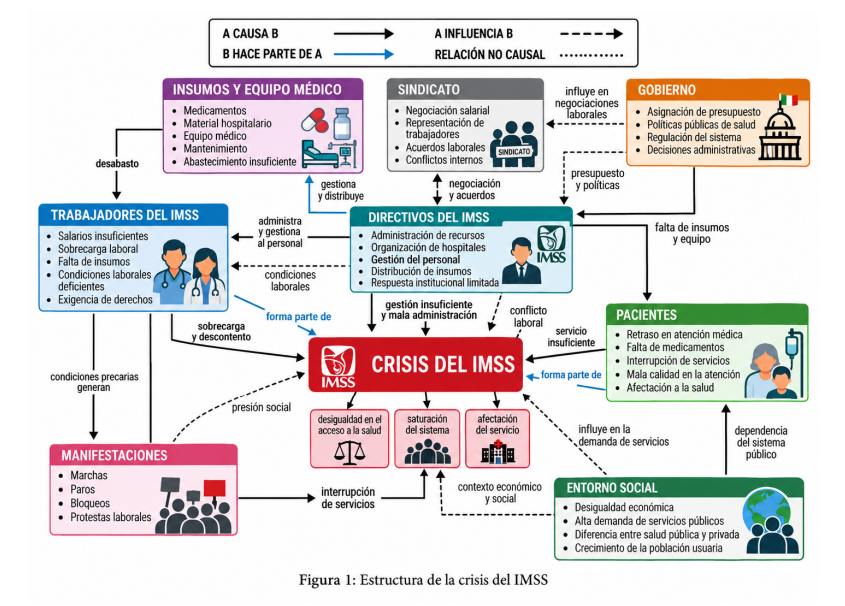
\includegraphics[width=\textwidth]{figura1.png}
\end{figure}

En este diagrama mostramos a los principales actores involucrados en la crisis del IMSS y cómo se relacionan entre ellos. Podemos observar que las decisiones del gobierno, la administración de recursos, las condiciones laborales y el abastecimiento de medicamentos están conectados. También identificamos cómo los problemas que enfrentan los trabajadores pueden afectar a los pacientes y generar manifestaciones.

\subsection*{d) Paradigmas, Modelos Mentales y Comportamientos:}

Los eventos de la punta del iceberg son causados por comportamientos humanos, los cuales son dictados por modelos mentales y paradigmas profundamente arraigados.

\textit{Instrucción: Analicen a los actores de su diagrama y definan bajo qué mentalidad operan. ¿Qué creencias sostienen el problema? (ej. <<Hay que pelear por los recursos escasos. Primero yo, después yo y al último yo>>, o <<siempre lo hemos hecho así>>).}

\begin{itemize}
  \item \textbf{Trabajadores del IMSS:} Operan bajo la mentalidad de \textit{<<si trabajamos y cumplimos con nuestras responsabilidades, debemos recibir un salario justo, materiales suficientes y condiciones dignas para poder trabajar y poder atender a los pacientes de manera adecuada>>}. Consideran que manifestarse es una forma de exigir que sus necesidades sean escuchadas y respetadas.

  \item \textbf{Dirigentes Sindicales:} Operan bajo la creencia de que <<los acuerdos que se están negociando son suficientes para representar y cumplir con las exigencias de los trabajadores>>. Cuando los trabajadores sienten que sus demandas no están siendo escuchadas, surge el conflicto entre ambas partes para exigir sus derechos.

  \item \textbf{Directivos del IMSS:} Actúan desde la mentalidad centrada en mantener el funcionamiento de la institución y administrar los recursos DISPONIBLES; ellos fungen bajo la idea de <<hay que ajustarse al presupuesto y a las reglas establecidas>>. El problema surge cuando las limitaciones administrativas no generan soluciones oportunas para las necesidades del personal.

  \item \textbf{Gobierno:} Pueden priorizar la organización del sistema de salud, los presupuestos y los cambios administrativos, bajo la creencia <<las reformas y acuerdos establecidos permitirán mejorar el servicio y cumplir las exigencias de los trabajadores>>. Sin embargo, si no se consideran TODAS las necesidades de los trabajadores o no se cumplen las necesidades en su TOTALIDAD bajo los acuerdos establecidos, pueden seguir o aumentar las inconformidades, intermitencia en el servicio y manifestaciones y paros laborales.

  \item \textbf{Pacientes:} Su mentalidad se centra en la necesidad de recibir atención médica oportuna y de calidad, bajo la idea de que <<necesitamos que haya personal médico para atendernos, abastecimiento de medicamentos y materiales para cuando lo necesitamos para que nos puedan atender dignamente>>. Sin embargo, al estar el sector de salud en manifestación, son uno de los sectores más afectados al no poder recibir atención debido a la falta de personal, retrasos o interrupciones en los servicios.
\end{itemize}

% =====================================================
\section*{Paso 3: Aterrizando el Problema. Perspectiva del Usuario y Límites}

\textbf{Centrarse en el afectado:} Redacten el problema desde la experiencia de quien lo sufre, no desde la herramienta tecnológica que falta. \textbf{Delimitar el Alcance:} Tracen las fronteras de su reto. Hagan una lista de variables fuera de su control y mapeen limitantes técnicas, éticas, de tiempo y de presupuesto.

\subsection*{1. Perspectiva del usuario:}

(Trabajadores del IMSS y pacientes)

Los trabajadores del IMSS enfrentan inconformidades relacionadas con el salario, condiciones laborales, falta de insumos y el reconocimiento de sus derechos, lo que genera inconformidad a la hora de trabajar, ya que consideran que el esfuerzo, la responsabilidad y las largas jornadas de trabajo, incluidos los turnos extra, no siempre se ven reflejados en un salario digno. Además, deben realizar sus labores en condiciones que pueden dificultar su desempeño, debido a la falta de medicamentos, materiales, equipo médico o instalaciones adecuadas para brindar una atención de calidad.

Por otra parte, los pacientes sufren las consecuencias de las protestas y las deficiencias del servicio al estar el servicio de salud en paro, pues las interrupciones ocasionadas por algunas manifestaciones pueden dificultar el acceso a consultas, tratamientos y medicamentos.

El problema consiste en lograr condiciones laborales dignas para los trabajadores del IMSS, con salarios justos, suficientes insumos médicos, instalaciones adecuadas y respeto a sus derechos, sin descuidar las necesidades de los pacientes.

\textbf{Límites del problema:}

\begin{itemize}
  \item \textbf{Variables fuera de nuestro control:} Presupuesto y decisiones del gobierno, leyes laborales, acuerdos sindicales, cambios en la organización del sistema de salud.
  \item \textbf{Limitantes de tiempo:} Negociaciones, contratación del personal y la compra de medicamentos requieren tiempo, por lo que no hay soluciones inmediatas.
  \item \textbf{Limitantes de presupuesto:} Los recursos económicos son limitados; el presupuesto que le dé el gobierno a la directiva se debe distribuir a varios sectores, como salarios, medicamentos, equipos médicos, mantenimiento del hospital e instalaciones de la misma.
  \item \textbf{Limitantes técnicas:} Falta de medicamentos, falta de equipo médico e instalaciones adecuadas y personal insuficiente pueden dificultar la atención de los pacientes.
  \item \textbf{Limitantes éticas:} Es necesario respetar los derechos de los trabajadores a manifestarse por sus derechos y, al mismo tiempo, proteger el derecho de los pacientes a recibir atención médica, especialmente en casos de emergencia.
\end{itemize}

\subsection*{2. Definición de Criterios de Éxito:}

\textbf{Cuantitativos} (metas propuestas por nosotros)
\begin{itemize}
  \item \textbf{Salarios:} Lograr un aumento salarial del 10\% para los trabajadores del IMSS.
  \item \textbf{Medicamentos:} Reducir en un 50\% los reportes por falta de medicamentos y materiales médicos.
  \item \textbf{Sobrecarga laboral:} Disminuir un 30\% las horas extras del personal médico.
  \item \textbf{Atención médica:} Reducir un 40\% los tiempos de espera de los pacientes.
  \item \textbf{Manifestaciones:} Disminuir un 50\% las protestas relacionadas con las condiciones laborales.
\end{itemize}

\textbf{Cualitativos}
\begin{itemize}
  \item Conseguir que los trabajadores se sientan escuchados y valorados.
  \item Mejorar las condiciones de trabajo del personal médico.
  \item Lograr que los pacientes se sientan satisfechos con la atención recibida.
  \item Mejorar la comunicación entre los trabajadores, sindicatos y directivos.
  \item Generar mayor confianza en los servicios públicos de salud.
\end{itemize}

\subsection*{3. La Declaración del Problema (Problem Statement):}

En México, los trabajadores del IMSS y del IMSS-Bienestar enfrentan problemas relacionados con los salarios, las condiciones laborales y la falta de medicamentos y materiales médicos. Entre 2023 y 2026 se han registrado manifestaciones en diferentes estados del país, incluyendo una marcha de aproximadamente 1,500 trabajadores en octubre de 2024 y al menos 189 empleados afectados por irregularidades de pago en enero de 2025. Estas situaciones generan inconformidad entre el personal de salud y dificultan sus labores, lo que también puede afectar la atención de los pacientes. Si estos problemas continúan, podrían aumentar los conflictos laborales y las dificultades para garantizar una atención médica adecuada.

% =====================================================
\section*{Paso 4: Evaluación de las <<Soluciones>> Actuales}

\textbf{Solución actual:} Propuesta de aumento salarial del 6.8\% para los trabajadores del IMSS.

En septiembre de 2026, los trabajadores del IMSS manifestaron su inconformidad con una propuesta de aumento salarial del 6.8\%, que incluía un 2.9\% directo al salario tabular y un 3.9\% en prestaciones. Los trabajadores rechazaron esta propuesta porque consideraron que el aumento directo a su salario era insuficiente y exigían un incremento del 10\%.

\textbf{¿Es deseable? (Factor humano)}

Consideramos que esta propuesta es parcialmente deseable porque busca mejorar los ingresos de los trabajadores. Sin embargo, muchos de ellos no estaban de acuerdo con el porcentaje ofrecido, ya que consideraban que no respondía a sus necesidades. Además, sus inconformidades no solamente estaban relacionadas con el salario, sino también con la falta de medicamentos, materiales médicos y mejores condiciones laborales.

\textbf{¿Es factible? (Desafío técnico y estructural)}

Consideramos que puede ser factible porque el IMSS y los representantes sindicales cuentan con mecanismos para negociar los salarios y las prestaciones. Sin embargo, aunque se lograra aplicar el aumento, esto no resolvería otros problemas que enfrentan los trabajadores, como la falta de personal, medicamentos y equipo médico. Por lo tanto, la propuesta solamente atiende una parte del problema.

\textbf{¿Es viable? (Ecosistema y sostenibilidad)}

Consideramos que podría ser viable si el IMSS cuenta con los recursos económicos necesarios para mantener el aumento salarial sin afectar el presupuesto destinado a medicamentos, instalaciones y atención médica. Sin embargo, no podemos asegurar que sea sostenible a largo plazo porque no contamos con información suficiente sobre sus costos. Además, esta medida no garantiza que mejoren las condiciones de los hospitales ni la atención que reciben los pacientes.

\subsection*{Reporte crítico: ¿Por qué esta solución no es suficiente?}

Después de analizar esta propuesta, consideramos que el aumento salarial del 6.8\% no era suficiente para atender todas las inconformidades de los trabajadores del IMSS. Aunque buscaba mejorar sus ingresos, no respondía completamente a sus exigencias salariales ni resolvía problemas como la falta de medicamentos, materiales médicos y personal. Esto demuestra que la propuesta presenta limitaciones en el factor humano y en el aspecto estructural, ya que no atiende todas las necesidades de los trabajadores ni las dificultades que enfrentan los hospitales.

Por esta razón, consideramos necesaria una futura intervención de ingeniería con una perspectiva sistémica, que permita analizar cómo se relacionan la administración de recursos, las condiciones laborales, el abastecimiento de medicamentos y la atención a los pacientes. De esta manera, se podría comprender mejor el problema en su conjunto, en lugar de atender únicamente una de sus causas.

\textbf{Fuente:}

Villaseñor, A. (2026, 25 de septiembre). Protestan trabajadores del IMSS contra aumento avalado por su sindicato. \textit{La Jornada}. \url{https://www.jornada.com.mx/2026/09/25/politica/012n1pol}

\nocite{*}
\bibliographystyle{plain}
\bibliography{documento}

\end{document}